\documentclass{noithesis}

\newtheorem{theorem}{定理}[section]
\newtheorem{definition}[theorem]{定义}
\newtheorem{lemma}[theorem]{引理}
\newtheorem{property}{性质}[theorem]


\begin{document}
	
	\title{2023 程序设计 II 荣誉课程大作业报告}
	\author{中国人民大学~~李修羽}
	
	\maketitle
	
	\begin{abstract}
		本文主要探究了基于 Qt 图形界面应用设计的不围棋联网对战软件制作过程,对一些重要功能的实现进行了说明,同时对于团队分工过程有一定记录。在联网体系之外,额外探究了不围棋 AI 的算法设计与实现。
	\end{abstract}

	\tableofcontents
	\setcounter{page}{0}
	\thispagestyle{empty}
	\newpage
	
	\section{团队构成}
	
	\subsection{闲话}
	
	理论上这个大作业一个人也可以做,但是既然都称之为团队大作业了,那就团队做。
	
	\subsection{小组分工}
	
	不知道现在是个什么分工。
	
	\section{Qt 图形界面应用设计}
	
	\subsection{UI 设计}
	
	\begin{figure}[!htb]{
		\centering
		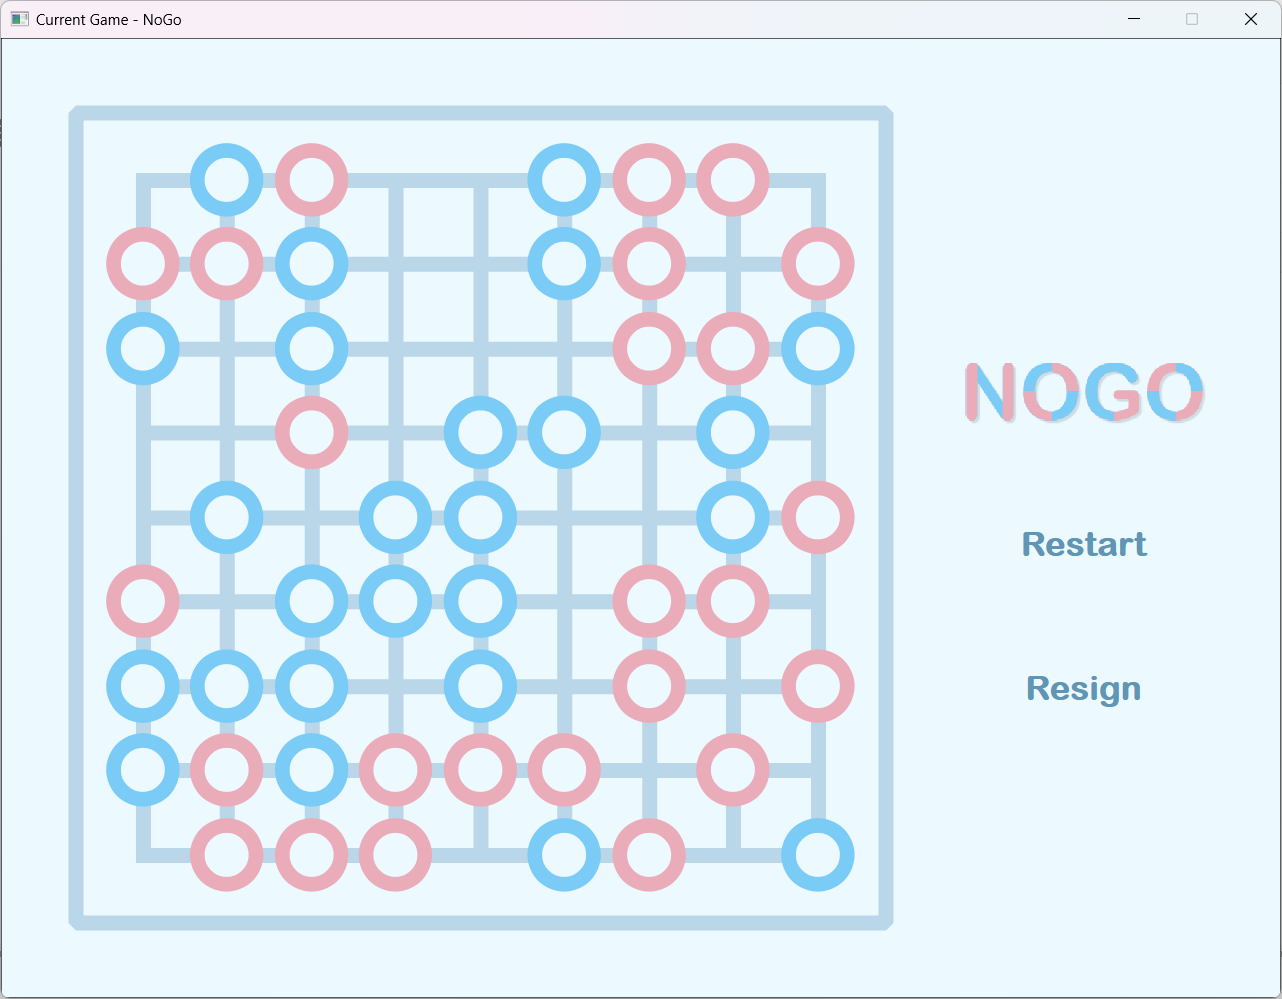
\includegraphics[width=0.8\textwidth]{img/UI.png}
			\counterwithin{figure}{section}
			\caption{随机 demo 示例}
	}
	\end{figure}

	本应用 UI 设计采用扁平化的设计风格,搭配上饱满、明亮、可爱且前卫的颜色设计,字体使用 Sans-serif 字体 Arial Rounded MT Bold,平衡现代感和亲和感,剩下的我编不下去了还没写,更多的 UI 设计还在写。

	\subsection{简单逻辑}
	
	在写了在写了
	
	\section{AI 算法设计}
	
	别卷了,还没写,你家程设就 $2$ 分。
	
	
\end{document}